\documentclass[a4paper,10pt,titlepage]{article}
% PREUMBULUM
\usepackage[utf8]{inputenc}
\usepackage[T1]{fontenc}

\usepackage{a4wide} 
\usepackage{times}

\usepackage[magyar,english]{babel}

% Forráskódoknak:
\usepackage{listings}

% Tartalomjegyzék:
\usepackage{tocbibind}

\usepackage[usenames,dvipsnames]{color}

% Hogy legyen képünk:
\usepackage{graphicx}

%###############################################################################
\newcommand{\szerzo}{\input{szerzok.inc}}
\newcommand{\cim}{Hallgatói előrehaladás támogató ''badge'' rendszer \\ Rendszerterv}
\newcommand{\cimmeta}{Hallgatói előrehaladás támogató ''badge'' rendszer - Rendszerterv}
\newcommand{\targy}{}
\newcommand{\kulcsszavak}{}

\usepackage{hyperref}
\hypersetup{
    unicode=true,
    colorlinks=true,
    linkcolor=RoyalBlue,
    citecolor=RoyalBlue,
    filecolor=RoyalBlue,
    urlcolor=RoyalBlue,
    pdftitle={\cimmeta},        % title
    pdfauthor={\szerzo},    % author
    pdfsubject={\targy}, % subject of the document
    pdfcreator={},   % creator of the document
    pdfproducer={LaTeX, TexMaker},    % producer of the document
    pdfkeywords={\kulcsszavak},    % list of keywords
}

\usepackage{url}

% Táblázatoknak:
\usepackage{colortbl}

% Ha kell matek:
\usepackage{amssymb,amsmath}

\usepackage{verbatim} % Hogy lehessen blokkkommentezni

% Egymás melleti képekhez:
\usepackage{subfig}

\setlength{\parindent}{12pt} % magyar nyelvű dokumentumokban jellemző
\setlength{\parskip}{0pt}    % magyar nyelvű dokumentumokban jellemző

\usepackage{setspace}  % Ettol a tablazatok, abrak, labjegyzetek maradnak 1-es sorkozzel!

%###########################################
% Saját eszközök:
%
\definecolor{todobgszin}{rgb}{0.64,0.78,0.22}
\definecolor{todofrszin}{rgb}{0.00,0.50,0.00}

\newcommand{\angolul}[1]{\foreignlanguage{english}{#1}}

\newcommand{\todo}[1]{
    \vfill
    \begingroup % Csinálunk egy csoportot, hogy az identálás csak erre vonatkozzon
        \setlength{\parindent}{0cm} % Beállítjuk, hogy teljes szélességű legyen a dobozunk a bekezdéstől függetlenül
        \fcolorbox{todofrszin}{todobgszin}{
            \parbox{\textwidth}{
                \vskip10pt
                \leftskip10pt
                \rightskip10pt
            
                \emph{TODO: #1}
  
                \vskip10pt
            }
        }
    \endgroup
    \vfill
}

\newenvironment{sajat_itemize}
{
	\begin{itemize}
	\setlength{\itemsep}{0pt}
}
{
	\end{itemize}
}

\begin{document}
% Dokumentumtörzs

\selectlanguage{magyar}

% Címoldal:
\begin{titlepage}

\title{\cim}
\author{\szerzo}
\date{\today}

\end{titlepage}
\maketitle

% Nem akarom, hogy megjelenjen a tartalomjegyzékben a Tartalomjegyzék:
\section*{Tartalomjegyzék}
\makeatletter
\@starttoc{toc}
\makeatother

\newpage

\section{Architektúra leírás}
A megvalósított rendszer egy rétegzett architekturális rendszer. A rétegek elválasztása funkcionális szempont alapján valósítottuk meg, három réteget különböztetünk meg:

\begin{sajat_itemize}
\item Megjelenítés
\item Alkalmazás
\item Adatbázis
\end{sajat_itemize}

\begin{figure}[ht!]
\centering
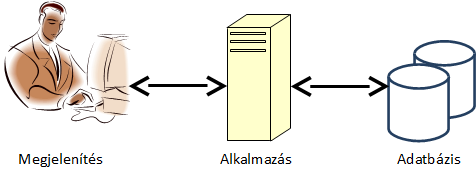
\includegraphics[width=0.80\textwidth]{figures/3tier.png}
\caption{A hátom rétegű architektúra \label{fig:3tier}}
\end{figure}

\subsection{Megjelenítés}
A felhasználó ezzel a réteggel áll interakcióban, ezen keresztül éri el a számára szükséges, illetve hozzáférhető adatokat, melyet a középső réteg, az alkalmazás nyújt számára. Cél, a felhasználói élmény minél magasabb fokú szolgáltatása. Ez úgy érhető el, hogy a felhasználó számára egy egyszerű, számára már jól ismert alkalmazáson, az általa választott és ismert web böngészőn keresztül, nyújtunk többletszolgáltatásokat.

\subsection{Alkalmazás}
A megjelenítési réteg számára nyújt szolgáltatást HTTP(S) protokollon keresztül, az adatbázis réteg felhasználásával.

Megvalósítása Python nyelven a Django keretrendszerrel történik, mely az alkalmazási rétegen belül MVC architektúrával épül fel. A View és a Controller is az alkalmazás réteghez tartozik, a megjelenítési réteg nincs tudatában, hogy a kiszolgálását két külön komponens végzi. A Controller fogadja a kéréseket, elkészíti a megjelenítendő adatot az adatbázisrétegből lekérdezve (vagy módosítja azt), majd egy View-ként átadja a megjelenítési rétegnek.

\subsection{Adatbázis}
Az adatbázis szerver SQLite adatbázis, mely tartalmazza a felhasználókat, szerepköreiket, a definiált célokat, feladatokat, badge-eket.

\section{Az architektúra előnyei}
A háromrétegű architektúra használatának legfőbb előnyei, hogy feladatkörök jól definiáltan elkülöníthetők, valamint az alkalmazás és az adatbázis szétválasztása jó megvalósítás esetén növeli a rendszer biztonságát.

\section{Alkalmazott model}

\begin{figure}[ht!]
\centering
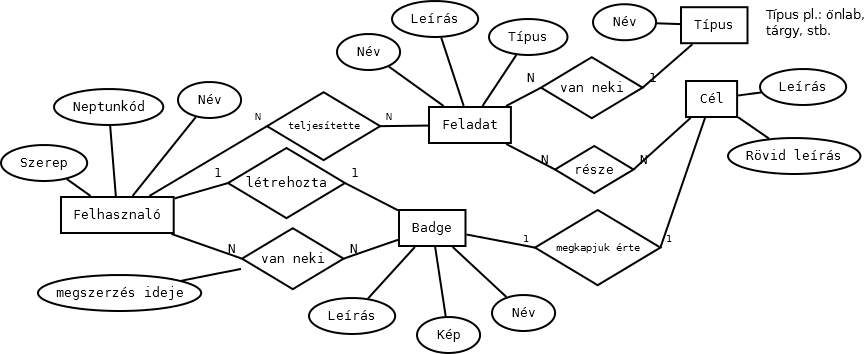
\includegraphics[width=1.00\textwidth]{figures/modell.png}
\caption{A rendszer ER modellje \label{fig:modell}}
\end{figure}

Egy Badge megszerzéséhez egy vagy több célt kell elérni. Egy cél tartalmazhat konkrét megvalósítandó feladatot, de lehet feladat típust is meghatározni.

\section{Felhasználói szerepek}
A felhasználó megjelenítheti saját adatait, elért badge-eit, valamint a még el nem ért badge-eket. Ezeket nyomtathatja is.
Az oktató hozzáfér egy korlátozott adminisztrációs felülethez, melyen definiálhat új feladatokat, badge-eket és célokat. 
Az adminisztrátor felelőssége új felhasználók felvétele valamint törlése a rendszerből.

\end{document}